\documentclass{article}
\usepackage{graphicx}  % Pour inclure des images
\usepackage[french]{babel}  % Pour la langue française
\usepackage[T1]{fontenc}
\usepackage{placeins}  % Encodage des caractères


\begin{document}

\title{Prototype }
\author{Tristan Petit, Nils Hubert, Toni Rey, \\ Majd El Sebeiti, Vianney Miquel}
\date{\today}

\maketitle

\section{Introduction}

Ce document regroupe un total de \textbf{n} captures d'écran accompagnées d'explications détaillées.

\section{Communication entre deux VM}

L'image ci-dessous illustre un ping entre la machine virtuelle de Toni et celle de Vianney, qui ne se trouvent pas sur le même hyperviseur.

\begin{figure}[h]
    \centering
    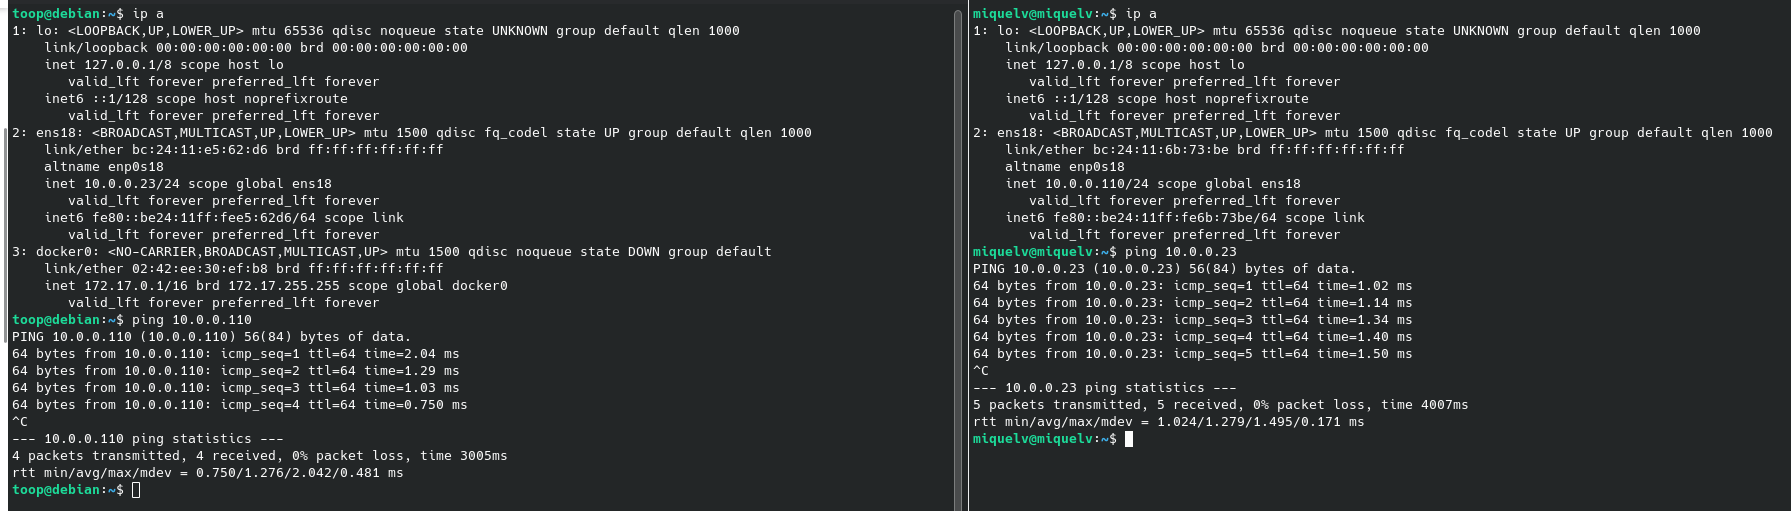
\includegraphics[width=1\textwidth]{Ping.png}
    \caption{Ping entre deux machines virtuelles sur des hyperviseurs distincts}
\end{figure}

\section{Interfaces du routeur et sous-réseaux}

Le routeur 10.0.0.1 est une machine virtuelle hébergée sur le proxmox de Vianney.
L'image suivante montre les interfaces du routeur d'entrée dans chaque sous-réseau de l'infrastructure. On a donc le sous-réseau 10.0.10.X, 10.0.20.X, 10.0.30X et 10.0.40.X pour les utilisateurs, administrateurs, serveurs de fichiers et DMZ respectivement.

\begin{figure}[h]
    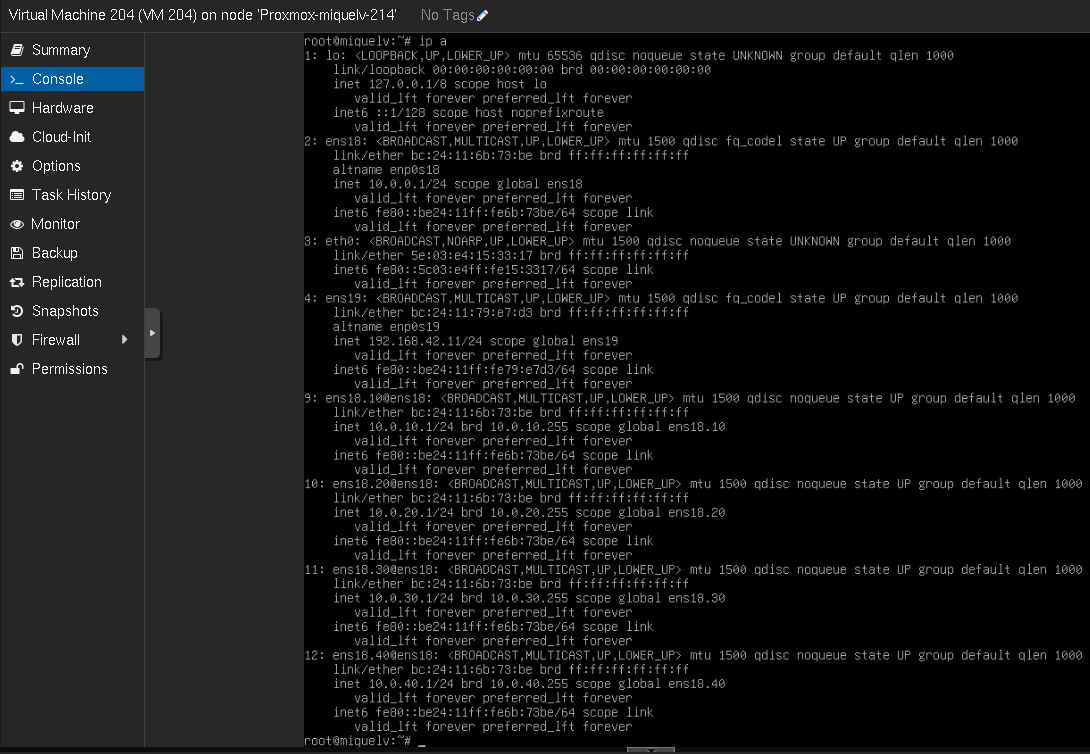
\includegraphics[width=\textwidth, keepaspectratio]{interfaces_routeur.png}
    \caption{Interfaces du routeur}
\end{figure}

\FloatBarrier

\section{Accès à Internet}

L'image suivante montre un ping du routeur vers google.com, prouvant qu'il peut accéder à internet. Suivi d'un ping vers une machine prototype du réseau, 10.0.0.23.

\begin{figure}[h]
    \centering
    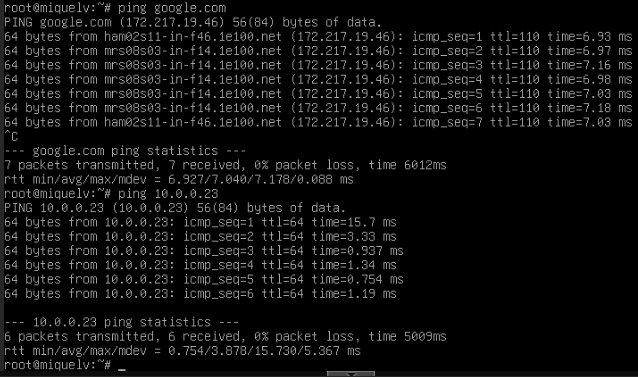
\includegraphics[width=1\textwidth]{router_ping.png}
    \caption{Test de connexion Internet et réseau local}
\end{figure}

\FloatBarrier

\section{Configuration du VXLan}

Les images suivantes montrent la création et configuration d'un VXLan qui nous permet de commuiquer entre les VM.

\begin{figure}[h]
    \centering
    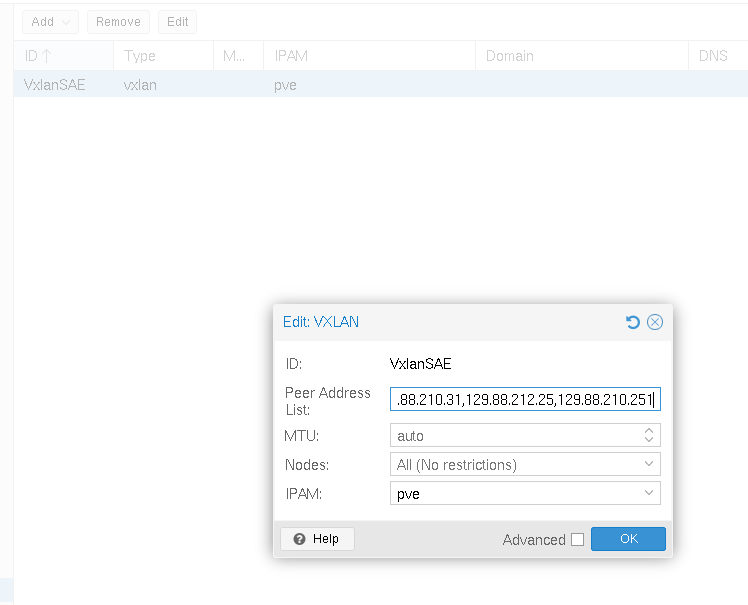
\includegraphics[width=1\textwidth]{VxLan.png}
    \caption{Création de la zone VXLAN}
\end{figure}

\FloatBarrier

\begin{figure}[h]
    \centering
    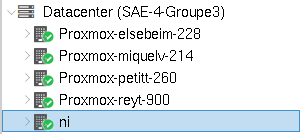
\includegraphics[width=1\textwidth]{Promox-1.png}
    \caption{Tous les proxmox sont dans le meme cluster}
\end{figure}

\FloatBarrier

\begin{figure}[h]
    \centering
    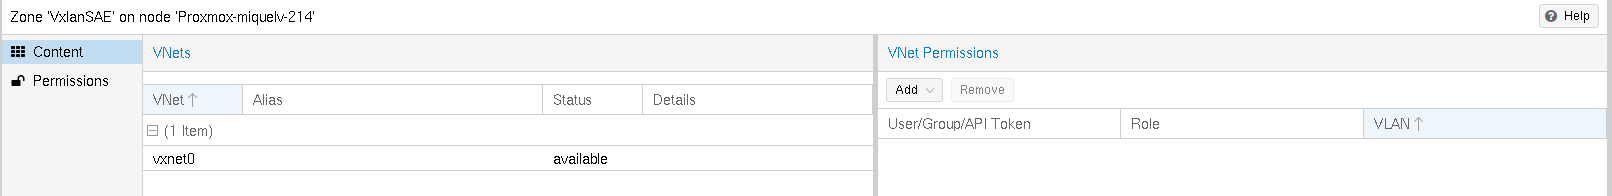
\includegraphics[width=1\textwidth]{VNets.png}
    \caption{Configuration du sous-réseau vxnet0}
\end{figure}

\FloatBarrier

\begin{figure}[h]
    \centering
    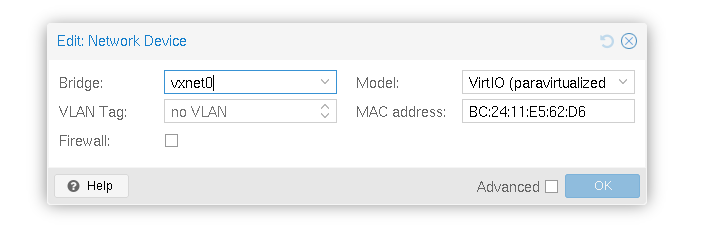
\includegraphics[width=1\textwidth]{VMtoni.png}
    \caption{Ajout du bridge vxnet0 sur une machine virtuelle}
\end{figure}

\FloatBarrier

\end{document}
